\chapter{المناعة التكيّفية والتلقيح}\label{ch:b3:adaptive-immunity}

في عام 1796 حكّ طبيب ريفي قيحًا من بثرة جدري بقر في ذراع
حلّابة فوضعه في ذراع صبي، ثم لقّحه بعد ستة أسابيع بالجدري؛
فلم يمرض الصبي. وفي عام 1980 أعلنت منظمة الصحة العالمية أن
الجدري --- الذي قتل ثلاثمئة مليون إنسان في القرن العشرين
--- قد استُؤصل من الأرض، بتلك الطريقة. والجهاز الذي جنّده
جينر، من غير أن يعلم بوجوده، يقدر على أن يتعرف أي جزيء لم
يلقه قط، وأن يختار من بين مئة مليار مستقبل مختلف القليلة
التي تلائم، وأن يضاعف الخلايا الحاملة لها مليون ضعف في
أسبوع، وأن يحسّن ملاءمتها بالطفر والانتخاب وهو يفعل ذلك،
وأن يتذكر النتيجة مدى العمر؛ وهو يتعلم أيضًا ألا يهاجم
الجسم الذي صنعه، وإخفاقاته في تعلم ذلك هي أمراض \omterm{def:b3:adaptive-immunity:tolerance}{المناعة
الذاتية}. ويتناول هذا الفصل اللمفاويات وكيف تصنع مستقبلاتها،
وكيف تُستنفر الاستجابة وتُحفظ، وكيف يُفرض التحمل ويُفقد،
والحساب الذي يجعل تلقيح عدد كافٍ من الناس يحمي من لم
يُلقَّحوا.

\section{اللمفاويات والانتخاب النسيلي}

\begin{definition}[اللمفاويات ومستقبلاتها]\label{def:b3:adaptive-immunity:lymphocytes}
\index{لمفاوية}\index{لمفاوية بائية}\index{لمفاوية تائية}\index{مستضد}\index{انتخاب نسيلي}\index{عقدة لمفية}
تحمل \emph{المناعةَ التكيّفية} \emph{اللمفاوياتُ}:
\emph{اللمفاويات البائية}، التي تنضج في نقي العظم ومستقبل
المستضد فيها \emph{\omterm{def:b3:adaptive-immunity:antibody}{ضد}} مثبت في الغشاء تفرزه لاحقًا؛
و\emph{اللمفاويات التائية}، التي تنضج في \omterm{def:b3:adaptive-immunity:tolerance}{التوتة} ويتعرف
مستقبلها شظايا ببتيدية معروضة على سطح خلايا أخرى.
و\emph{المستضد} كل ما يربطه مستقبل؛ والجزء الذي يُلامَس
فعلًا هو \emph{الحاتمة}. والحقيقة المؤسِّسة هي
\emph{الانتخاب النسيلي} (برنت، 1957): فكل لمفاوية تحمل
مستقبلات ذات نوعية واحدة فقط، مثبتة قبل أن تلقى أي مستضد؛
ويحوي الجسم ذخيرة من نحو $10^{11}$ خلية كهذه؛ وينتخب
المستضد القليلات التي تلائم مستقبلاتُها فيدفعها إلى الانقسام
إلى نسيلة من خلايا منفِّذة وخلايا ذاكرة؛ وتُحذف اللمفاويات
التي تلائم مستقبلاتها جزيئات الجسم نفسه أو تُسكَت وهي
تنضج. وتدور الخلايا دورانًا مستمرًا بين الدم و\emph{العقد
اللمفية} والطحال والنسيج اللمفي المخاطي، حيث يُعرض المستضد
الذي تحمله الخلايا التغصنية (\cref{ch:b3:innate-immunity})،
فتجده الخلية الملائمة النادرة --- واحدة في مئة ألف لحاتمة
بعينها --- في يوم أو يومين.
\end{definition}

\begin{proof}[شواهد]
وضع نوسال وليدربرغ (1958) لمفاويات مفردة من جرذان مُمنَّعة
في قُطيرات مجهرية واختبرا \omterm{def:b3:adaptive-immunity:antibody}{الضد} الذي تفرزه كل واحدة: فكانت
كل خلية تصنع ضدًا لأحد المستضدين، لا لكليهما قط. وكان برنت
قد تنبأ بذلك في السنة السابقة. وقارن تونيغاوا (1976) DNA
مورّثة \omterm{def:b3:adaptive-immunity:antibody}{ضد} في خلايا جنينية وفي \omterm{def:b3:cancer-biology:hallmarks}{ورم} مفرز للأضداد: ففي الجنين
كان الجزآن المتغير والثابت متباعدين، وفي \omterm{def:b3:cancer-biology:hallmarks}{الورم} كانا
موصولين --- فقد قُطعت المورّثة ووُصلت في الخلية الجسدية،
وذلك أول برهان على جينوم يُعاد ترتيبه عمدًا.
\end{proof}

\section{صنع مئة مليار مستقبل}

\begin{definition}[بنية الضد وإعادة تركيب V(D)J]\label{def:b3:adaptive-immunity:antibody}
\index{ضد}\index{غلوبولين مناعي}\index{إعادة تركيب V(D)J}\index{RAG}\index{تنوع وصلي}\index{تبديل الصنف}
\emph{الضد} (الغلوبولين المناعي) سلسلتان ثقيلتان متطابقتان
وسلسلتان خفيفتان متطابقتان، في كل منها نطاق \emph{متغير} في
طرفها ونطاقات \emph{ثابتة} وراءه؛ ويربط كل ذراع من الذراعين
حاتمةً بثلاث عُرى شديدة التغير من النطاق المتغير الثقيل
وثلاث من الخفيف، والساق (Fc) هي ما تتعرفه البالعات \omterm{def:b3:innate-immunity:complement}{والمتمّمة}
والخلايا البدينة. وتختلف خمسة أصناف في المنطقة الثابتة من
سلسلتها الثقيلة: IgM، وهو أول ما يُصنع، خماسي يفعّل \omterm{def:b3:innate-immunity:complement}{المتمّمة}
تفعيلًا جيدًا؛ وIgG، حصان عمل الدم والنسج، وهو يعبر
المشيمة؛ وIgA، ثنائي يُفرز عبر الأسطح المخاطية إلى الأمعاء
والطرق الهوائية والحليب؛ وIgE، ترتبط به الخلايا البدينة،
وهو ضد الديدان --- وسبب الأرجية؛ وIgD. والنطاقات المتغيرة
ليست مرمَّزة كما هي. فموضع السلسلة الثقيلة يحوي نحو $40$
قطعة \emph{V} عاملة، و$25$ قطعة \emph{D}، و$6$ قطع \emph{J}؛
وتختار \omterm{def:b3:adaptive-immunity:lymphocytes}{اللمفاوية البائية} النامية واحدة من كل نوع وتصلها
\emph{بإعادة تركيب V(D)J}: إذ يقطع الإنزيمان RAG1 وRAG2 عند
متواليات إشارة إعادة التركيب المحيطة بالقطع، وتُوصل النهايات
بآلة الوصل الطرفي غير المتماثل في \cref{ch:b3:dna-repair}،
مع تشذيب نوكليوتيدات وإضافتها عشوائيًا (بالإنزيم TdT) عند
كل وصلة --- وذلك \emph{التنوع الوصلي}، الذي يقع بالضبط في
العروة الثالثة الشديدة التغير. وتفعل السلاسل الخفيفة الشيء
نفسه مع V وJ. وبعد بدء الاستجابة يُوصل النطاق المتغير نفسه
بمنطقة ثابتة مختلفة بإعادة ترتيب ثانية هي \emph{تبديل
الصنف}، فتتغير وظيفة الضد لا نوعيته.
\end{definition}

\begin{theorem}[حجم الذخيرة]\label{thm:b3:adaptive-immunity:repertoire}
\index{ذخيرة!توفيقية}
عند $V_{H} = 40$، و$D = 25$، و$J_{H} = 6$ قطعًا ثقيلة، وسلاسل
خفيفة من موضعين عند $(V_{\kappa}, J_{\kappa}) = (40, 5)$
و$(V_{\lambda}, J_{\lambda}) = (30, 4)$، يكون عدد التوافيق
الثقيلة--الخفيفة المتمايزة التي تُنال باختيار القطع وحده
\[
(40\times 25\times 6)\times(40\times 5 + 30\times 4) = 6000\times 320
= 1.9\times 10^{6}.
\]
ويضرب \omterm{def:b3:adaptive-immunity:antibody}{التنوع الوصلي} عند الوصلتين الثقيلتين والوصلة الخفيفة
هذا العدد بعامل من رتبة $10^{4}$--$10^{5}$، فتُعطى ذخيرة
ممكنة فوق $10^{10}$ من أقل من $200$ قطعة مورّثية --- أي أكثر
من عدد اللمفاويات البائية في الجسم، فتكون الذخيرة الفعلية
عينة من الذخيرة الممكنة. ثم يولّد \omterm{def:b3:adaptive-immunity:germinal-centre}{الطفور الجسدي المفرط}
أثناء الاستجابة (أدناه) متغيرات من كل مستقبل منتخَب.
\end{theorem}
\begin{proof}
كل سلسلة ثقيلة هي V واحدة وD واحدة وJ واحدة؛ وكل سلسلة
خفيفة V واحدة وJ واحدة من أي من الموضعين؛ وتقترن أي ثقيلة
بأي خفيفة، فتتضارب الأعداد (مبدأ الضرب)، ويتجامع الموضعان
الخفيفان. والعامل الوصلي هو عدد المتواليات المتمايزة التي
يقدر التشذيب والإضافة العشوائيان على إنتاجها عند وصلة ---
بضع عشرات لكل وصلة على الأقل --- مرفوعًا إلى عدد الوصلات؛
وقيمته بالضبط غير محددة، غير أن ثلاث وصلات لكل منها
$30$--$50$ نتيجة تعطي من $3\times 10^{4}$ إلى $10^{5}$. وعدد
مستقبلات اللمفاويات التائية، بسلسلتين يُعاد ترتيبهما
بالطريقة نفسها وبإسهام وصلي أكبر، من الرتبة نفسها.
\end{proof}

\begin{omfigure}
\begin{tikzpicture}[every node/.style={font=\scriptsize}, >=stealth]
  % antibody Y
  \begin{scope}[xshift=0cm]
    % heavy chains
    \draw[very thick, omDef] (0,0) -- (0,1.6) -- (-1.3,3.0); \draw[very thick, omDef] (0.35,0) -- (0.35,1.6) -- (1.65,3.0);
    % light chains
    \draw[very thick, omProp] (-0.45,1.55) -- (-1.75,2.95); \draw[very thick, omProp] (0.8,1.55) -- (2.1,2.95);
    \fill[omThm] (-1.55,3.0) circle (0.12); \fill[omThm] (1.9,3.0) circle (0.12);
    \node[above, align=center] at (-1.5,3.15) {النطاقات المتغيرة:\\موقع ربط المستضد}; 
    \node[right, align=left] at (0.55,0.5) {ساق Fc (ثابتة):\\الصنف يقرر الوظيفة};
    \node[left, omProp] at (-0.7,2.1) {خفيفة}; \node[right, omDef] at (0.4,1.3) {ثقيلة};
    \draw[omDef] (0.05,1.1) -- (0.3,1.1); \draw[omDef] (0.05,0.7) -- (0.3,0.7);
  \end{scope}
  % V(D)J locus
  \begin{scope}[xshift=4.2cm, yshift=2.4cm, xscale=0.86]
    \draw[very thick, gray] (0,0) -- (8.2,0);
    \foreach \x in {0.2,0.6,1.0,1.4} \draw[thick, fill=omDef!40] (\x,-0.15) rectangle (\x+0.3,0.15);
    \node[above] at (0.95,0.2) {قطع V ($\sim 40$)}; \node[font=\tiny] at (1.95,0) {$\cdots$};
    \foreach \x in {2.5,2.8,3.1} \draw[thick, fill=omProp!50] (\x,-0.15) rectangle (\x+0.2,0.15);
    \node[above] at (2.9,0.2) {D ($25$)};
    \foreach \x in {3.8,4.1,4.4} \draw[thick, fill=omMeth!50] (\x,-0.15) rectangle (\x+0.2,0.15);
    \node[above] at (4.2,0.2) {J ($6$)};
    \foreach \x/\lab in {5.3/\mu,6.0/\delta,6.7/\gamma,7.4/\alpha} { \draw[thick, fill=gray!30] (\x,-0.15) rectangle (\x+0.5,0.15); \node[above] at (\x+0.25,0.2) {C$_{\lab}$}; }
    \draw[->, thick] (4.1,-0.4) -- (4.1,-1.1) node[midway, right, align=left, font=\tiny] {RAG يقطع عند متواليات الإشارة؛ وتُوصل V واحدة وD واحدة،\\وJ واحدة، ويضيف TdT نوكليوتيدات عشوائية};
    % rearranged
    \draw[very thick, gray] (0,-1.5) -- (3.3,-1.5);
    \draw[thick, fill=omDef!40] (1.0,-1.65) rectangle (1.3,-1.35); \fill[omThm] (1.3,-1.65) rectangle (1.4,-1.35);
    \draw[thick, fill=omProp!50] (1.4,-1.65) rectangle (1.6,-1.35); \fill[omThm] (1.6,-1.65) rectangle (1.7,-1.35);
    \draw[thick, fill=omMeth!50] (1.7,-1.65) rectangle (1.9,-1.35);
    \draw[thick, fill=gray!30] (2.6,-1.65) rectangle (3.1,-1.35); \node[above] at (2.85,-1.3) {C$_{\mu}$};
    \node[below, align=center] at (1.45,-1.7) {VDJ موصولة: النطاق المتغير،\\بالأحمر: النوكليوتيدات الوصلية};
    \node[right, align=left, font=\tiny] at (3.4,-2.0) {مشذَّبة إلى C$_{\mu}$: سلسلة ثقيلة IgM؛\\وتبديل الصنف لاحقًا يصل VDJ نفسها\\إلى C$_{\gamma}$ أو C$_{\alpha}$};
  \end{scope}
\end{tikzpicture}

{\small يسارًا: \omterm{def:b3:adaptive-immunity:antibody}{ضد} --- سلسلتان ثقيلتان وسلسلتان خفيفتان،
والنطاقات المتغيرة في الأطراف تكوّن موقعي ربط، والساق
الثابتة يقرؤها سائر الجهاز المناعي. ويمينًا: موضع السلسلة
الثقيلة قبل \omterm{def:b3:adaptive-immunity:antibody}{إعادة تركيب V(D)J} وبعدها، وهي تنتقي قطعة من كل
نوع وتضيف نوكليوتيدات عشوائية عند الوصلات.}
\end{omfigure}

\begin{definition}[مستقبلات اللمفاويات التائية وMHC]\label{def:b3:adaptive-immunity:mhc}
\index{مستقبل لمفاوية تائية}\index{معقد التوافق النسيجي الكبير}\index{عرض المستضد}\index{التقييد بمعقد التوافق}\index{HLA}
\emph{مستقبل \omterm{def:b3:adaptive-immunity:lymphocytes}{اللمفاوية التائية}} جزيء من سلسلتين مبني بإعادة
التركيب نفسها، لا يُفرز أبدًا، ولا يربط مستضدًا حرًّا في
المحلول: بل يتعرف ببتيدًا قصيرًا محمولًا في أخدود جزيء من
\emph{معقد التوافق النسيجي الكبير} (MHC) على سطح خلية أخرى.
و\emph{MHC من الصنف~I}، الموجود على كل خلية ذات نواة، يعرض
ببتيدات من ثمانية إلى عشرة بقايا يقطعها البروتيازوم من
بروتينات الخلية نفسها في عصارتها --- وهي عينة مما تصنعه
الخلية، بما في ذلك أي \omterm{def:b3:virology:virus}{فيروس} --- على اللمفاويات التائية
\emph{CD8}، التي تقتل الخلية إن كان الببتيد غريبًا.
و\emph{MHC من الصنف~II}، على الخلايا التغصنية والبلعميات
واللمفاويات البائية، يعرض ببتيدات من ثلاثة عشر إلى خمسة
وعشرين بقية من بروتينات التقطتها الخلية وهضمتها في جسيمات
داخلية، على اللمفاويات التائية \emph{CD4}، التي تستجيب
بالمساعدة. \omterm{def:b3:adaptive-immunity:lymphocytes}{واللمفاوية التائية} \emph{مقيَّدة}: فهي لا تتعرف
ببتيدها إلا على أليل MHC الذي انتُخبت عليه. ومورّثات MHC
(\emph{HLA} في الإنسان) أشد مورّثات الجينوم تعددَ أشكال،
فيها آلاف الأليلات يختلف كل منها في الأخدود، فيعرض كل شخص
عينة مختلفة من ببتيدات كل بروتين ولا يقدر ممرض على الإفلات
من العرض عند الجميع --- ولذلك أيضًا يُتعرف عضو مزروع من
متبرع غير مطابق غريبًا لدى نسبة كبيرة من لمفاويات المتلقي
التائية.
\end{definition}

\begin{proof}[شواهد]
أخمج زينكرناغل ودورتي (1974) فئرانًا من سلالتين نقيتين
\omterm{def:b3:virology:virus}{بفيروس} واختبرا لمفاوياتهما التائية السامة على خلايا هدف
مصابة: فقتلت اللمفاويات التائية الخلايا المصابة من سلالتها
هي لا من السلالة الأخرى، مع أن \omterm{def:b3:virology:virus}{الفيروس} كان واحدًا. فلم ترَ
\omterm{def:b3:adaptive-immunity:lymphocytes}{اللمفاوية التائية} \omterm{def:b3:virology:virus}{الفيروس} إلا مع جزيء MHC ذاتي ---
\emph{\omterm{def:b3:adaptive-immunity:mhc}{التقييد بمعقد التوافق}} --- وهو ما فُسِّر لاحقًا حين
أظهرت البنية البلورية لجزيء MHC (بيوركمان، 1987) أخدودًا
فيه ببتيد، وحين تبيّن أن \omterm{def:b3:adaptive-immunity:mhc}{مستقبل اللمفاوية التائية} يربط
الاثنين معًا.
\end{proof}

\begin{omfigure}
\begin{tikzpicture}[every node/.style={font=\scriptsize}, >=stealth]
  % class I pathway
  \begin{scope}
    \draw[thick, omDef, fill=omDef!8] (0,0) rectangle (6.2,3.6); \node[anchor=north west] at (0.05,3.55) {أي خلية ذات نواة};
    \node[draw, rounded corners, fill=omThm!20, font=\tiny, align=center] (v) at (1.4,2.6) {بروتين فيروسي أو ذاتي\\في العصارة الخلوية};
    \node[draw, rounded corners, fill=gray!20, font=\tiny, align=center] (p) at (1.4,1.5) {البروتيازوم:\\ببتيدات من 8--10};
    \node[draw, rounded corners, fill=omDef!25, font=\tiny, align=center] (er) at (4.6,1.5) {الشبكة الباطنة: تُحمَّل\\على MHC الصنف I};
    \draw[->, thick] (v) -- (p); \draw[->, thick] (p) -- node[midway, above, font=\tiny] {TAP} (er);
    \draw[->, thick] (er) -- (4.6,3.55);
    \draw[thick, fill=omDef!40] (4.4,3.6) rectangle (4.8,4.1); \fill[omThm] (4.6,4.2) circle (0.09);
    \node[above, align=center] at (4.6,4.35) {ببتيد--MHC I\\تراه اللمفاويات التائية CD8: قتل};
  \end{scope}
  % class II pathway
  \begin{scope}[xshift=7.2cm]
    \draw[thick, omProp, fill=omProp!8] (0,0) rectangle (6.2,3.6); \node[anchor=north west] at (0.05,3.55) {خلية تغصنية، وبلعمية، ولمفاوية بائية};
    \node[draw, rounded corners, fill=omThm!20, font=\tiny, align=center] (ex) at (1.4,2.6) {بروتين مُلتقَط\\في جسيم داخلي};
    \node[draw, rounded corners, fill=gray!20, font=\tiny, align=center] (dig) at (1.4,1.5) {مهضوم:\\ببتيدات من 13--25};
    \node[draw, rounded corners, fill=omProp!30, font=\tiny, align=center] (m2) at (4.6,1.5) {MHC الصنف II\\يُحمَّل هنا};
    \draw[->, thick] (ex) -- (dig); \draw[->, thick] (dig) -- (m2);
    \draw[->, thick] (m2) -- (4.6,3.55);
    \draw[thick, fill=omProp!50] (4.4,3.6) rectangle (4.8,4.1); \fill[omThm] (4.6,4.2) circle (0.09);
    \node[above, align=center] at (4.6,4.35) {ببتيد--MHC II\\تراه اللمفاويات التائية CD4: مساعدة};
  \end{scope}
\end{tikzpicture}

{\small سبيلا العرض. الصنف~I يُري اللمفاويات التائية CD8 ما
تصنعه الخلية في داخلها؛ والصنف~II يُري اللمفاويات التائية
CD4 ما أكلته خلية عارضة \omterm{def:b3:adaptive-immunity:lymphocytes}{للمستضد}. فالاستجابة السامة تصوَّب
إلى الأول، والاستجابة المساعدة إلى الثاني.}
\end{omfigure}

\section{الاستجابة}

\begin{definition}[التفعيل، والمساعدة، والقتل]\label{def:b3:adaptive-immunity:response}
\index{لمفاوية تائية مساعدة}\index{لمفاوية تائية سامة}\index{تحفيز مشارك}\index{لمفاوية تائية نظيمية}\index{خلية بلازمية}\index{خلية ذاكرة}
تُفعَّل \omterm{def:b3:adaptive-immunity:lymphocytes}{اللمفاوية التائية} الساذجة حين يربط مستقبلها
ببتيد--MHC على \omterm{def:b3:innate-immunity:innate}{خلية تغصنية} توفر معه تحفيزًا مشاركًا
(\cref{ch:b3:innate-immunity})؛ ثم تنقسم كل ست إلى ثماني
ساعات أسبوعًا وتتمايز. فاللمفاويات التائية \emph{المساعدة
CD4} تتمايز، بحسب سيتوكينات \omterm{def:b3:innate-immunity:innate}{الخلية التغصنية}، إلى طوائف:
Th1، التي تفعّل البلعميات لتقتل ما أكلته (السل)؛ وTh2، التي
تسوق IgE والخلايا الحمضية \omterm{def:b3:adaptive-immunity:antibody}{ضد} الديدان؛ وTh17، التي تجنّد
العدلات \omterm{def:b3:adaptive-immunity:antibody}{ضد} البكتيريا والفطور خارج الخلوية؛ والمساعدات
الجريبية، التي تساعد اللمفاويات البائية؛ واللمفاويات
التائية \emph{النظيمية}، التي تكبت. واللمفاويات التائية
\emph{السامة CD8} تقتل الخلايا التي تعرض ببتيدها على
الصنف~I، بالبرفورين والغرانزيمات وبرابطة Fas، فتطلق
\omterm{def:b3:cell-cycle-apoptosis:apoptosis}{الاستماتة} (\cref{ch:b3:cell-cycle-apoptosis}) --- وهي الدفاع
\omterm{def:b3:adaptive-immunity:antibody}{ضد} الفيروسات والأورام. وتُفعَّل \omterm{def:b3:adaptive-immunity:lymphocytes}{اللمفاوية البائية} بارتباط
\omterm{def:b3:adaptive-immunity:lymphocytes}{المستضد} بمستقبلها مع مساعدة من \omterm{def:b3:adaptive-immunity:lymphocytes}{لمفاوية تائية} مساعدة جريبية
تتعرف ببتيدات \omterm{def:b3:adaptive-immunity:lymphocytes}{المستضد} نفسه على الصنف~II في \omterm{def:b3:adaptive-immunity:lymphocytes}{اللمفاوية
البائية}؛ فتصير عندئذ \emph{خلية بلازمية} تفرز آلاف الأضداد
في الثانية، أيامًا (قصيرة العمر، في العقدة) أو سنين (طويلة
العمر، في النقي)، أو تدخل مركزًا إنتاشيًا. واللمفاويات
البائية والتائية \emph{الذاكرة} --- طويلة العمر، أكثر عددًا
من سلائفها الساذجة وأسرع استجابةً --- هي بقية كل استجابة
وأساس التلقيح.
\end{definition}

\begin{definition}[المركز الإنتاشي]\label{def:b3:adaptive-immunity:germinal-centre}
\index{مركز إنتاشي}\index{طفور جسدي مفرط}\index{نضج الألفة}
في \emph{المركز الإنتاشي}، وهو بنية تتكون في \omterm{def:b3:adaptive-immunity:lymphocytes}{عقدة لمفية} بعد
أسبوع من بدء الاستجابة، تشغّل اللمفاويات البائية المفعَّلة
خوارزمية تطورية. ففي منطقته الداكنة تنقسم كل ست ساعات
وتُطفَّر مورّثات نطاقها المتغير بالإنزيم AID بمعدل نحو
تغيّر واحد لكل ألف زوج أساس في الانقسام --- وذلك
\emph{الطفور الجسدي المفرط}، وهو مليون ضعف المعدل الجينومي،
مصوَّب إلى كيلو أساس واحد. وفي المنطقة الفاتحة تختبر كل
خلية مستقبلها الجديد على \omterm{def:b3:adaptive-immunity:lymphocytes}{مستضد} محمول على خلايا تغصنية
جريبية وتنافس على مساعدة اللمفاويات التائية: فالخلايا التي
تربط ربطًا أفضل تلتقط مستضدًا أكثر، وتعرض أكثر، وتنال
مساعدة أكثر، وترجع إلى المنطقة الداكنة لتنقسم من جديد؛
والخلايا التي تربط ربطًا أسوأ، أو فقدت الربط، تموت
استماتةً. وعلى مدى أسبوعين إلى ثلاثة من الدورات ترتفع ألفة
الأضداد الناجية مئة إلى ألف ضعف --- وذلك \emph{نضج الألفة}
--- ويخرج الفائزون خلايا بلازمية وخلايا ذاكرة، وقد بدّلوا
صنفهم أيضًا. والاستجابة الثانوية أسرع وأكبر ومصنوعة من \omterm{def:b3:adaptive-immunity:antibody}{ضد}
أفضل لأنها تبدأ من هذه الجمهرة المنتخَبة الموسَّعة
المبدَّلة.
\end{definition}

\begin{omfigure}
\begin{tikzpicture}[every node/.style={font=\scriptsize}, >=stealth]
  \draw[thick, omDef, fill=omDef!12] (0,0) ellipse (2.7 and 1.7); \node[above, omDef!70!black] at (0,1.75) {المنطقة الداكنة};
  \draw[thick, omMeth!70!black, fill=omMeth!12] (6.2,0) ellipse (2.7 and 1.7); \node[above, omMeth!60!black] at (6.2,1.75) {المنطقة الفاتحة};
  \node[align=center] at (0,0.3) {تنقسم اللمفاويات البائية كل \qty{6}{h}؛\\ويطفّر AID مورّثات الضد:\\$10^{-3}$ لكل زوج أساس في الانقسام};
  \node[align=center] at (6.2,0.3) {اختبار المستقبل الجديد\\على مستضد تحمله\\خلايا تغصنية جريبية؛\\والتنافس على مساعدة التائيات};
  \draw[->, very thick, omProp] (2.4,0.7) .. controls (3.6,1.4) and (4.2,1.4) .. (3.7,0.7); \node[above, omProp] at (3.1,1.45) {الطافرات إلى الخارج};
  \draw[->, very thick, omMeth!70!black] (3.7,-0.7) .. controls (4.2,-1.4) and (3.6,-1.4) .. (2.4,-0.7); \node[below, omMeth!70!black] at (3.1,-1.45) {الفائزات راجعة، لتنقسم من جديد};
  \draw[->, thick, omThm] (6.6,-1.6) -- (6.6,-2.3); \node[below, omThm, align=center] at (6.6,-2.3) {الخاسرات: استماتة\\(معظمها)};
  \draw[->, thick] (8.9,0) -- (9.5,0); \node[right, align=left] at (9.5,0) {بعد 2--3 أسابيع:\\خلايا بلازمية (طويلة العمر،\\في النقي) وخلايا\\ذاكرة بائية؛ والألفة\\أعلى $100$--$1000\times$، مع تبديل الصنف};
\end{tikzpicture}

{\small \omterm{def:b3:adaptive-immunity:germinal-centre}{المركز الإنتاشي} آلةً تطورية: طفر في المنطقة
الداكنة، وانتخاب في المنطقة الفاتحة، ودوران بينهما حتى تربط
الأضداد الخارجة ربطًا أفضل بكثير من ربط الداخلة.}
\end{omfigure}

\begin{example}[حركية استجابة]\label{ex:b3:adaptive-immunity:kinetics}
نحو \omterm{def:b3:adaptive-immunity:lymphocytes}{لمفاوية بائية} واحدة في $10^{5}$ تربط حاتمة بعينها،
فتحوي اللمفاويات البائية $10^{11}$ التي في الجسم نحو $10^{6}$
سليفة، لعل مئة منها تلقى \omterm{def:b3:adaptive-immunity:lymphocytes}{المستضد} في العقدة النازحة. وبانقسام
كل ثماني ساعات تصير مئة خلية $10^{2}\times 2^{21} \approx 2\times 10^{8}$
في أسبوع. ويظهر \omterm{def:b3:adaptive-immunity:antibody}{الضد} في المصل بعد أربعة إلى ستة أيام، IgM
أولًا، ويبلغ ذروته بعد أسبوعين تقريبًا، ثم يتناقص بعمر نصف
قدره ثلاثة أسابيع بالنسبة إلى IgG إذ تموت الخلايا البلازمية
القصيرة العمر، فيستقر عند المستوى الذي تصونه الخلايا
البلازمية الطويلة العمر في النقي سنين. والتعرض الثاني يبدأ
من $10^{4}$--$10^{5}$ \omterm{def:b3:adaptive-immunity:response}{خلية ذاكرة} عالية الألفة مبدَّلة إلى
IgG فعلًا: فيرتفع \omterm{def:b3:adaptive-immunity:antibody}{الضد} في غضون يومين، أعلى بعشرة إلى مئة
ضعف، ويعادل الممرض قبل أن يستقر --- وذلك ما يشتريه \omterm{def:b3:adaptive-immunity:vaccine}{اللقاح}.
\end{example}

\begin{omfigure}
\begin{tikzpicture}
\begin{axis}[
  width=0.7\linewidth, height=5.6cm,
  axis x line=bottom, axis y line=left,
  xmin=0, xmax=70, ymin=1, ymax=10000, ymode=log,
  xlabel={أيام}, ylabel={ضد المصل (نسبي)},
  xlabel style={font=\small, at={(axis description cs:0.5,-0.12)}, anchor=north}, ylabel style={font=\small},
  tick label style={font=\small}, xtick={0,10,20,30,40,50,60,70},
  clip=false,
]
\addplot[very thick, omDef, domain=0:40, samples=60] {1 + 100*exp(-((x-14)/5)^2) + 15*(1-exp(-x/10))*exp(-(x-14)/60)*(x>14)};
\addplot[very thick, omThm, domain=40:70, samples=60] {1 + 2500*exp(-((x-48)/5)^2) + 400*(1-exp(-(x-40)/4))*(x>40)};
\draw[->, thick, gray] (axis cs:0,0.6) -- (axis cs:0,1.8); \node[font=\scriptsize, gray, anchor=south west] at (axis cs:0.5,1.3) {التعرض الأول};
\draw[->, thick, gray] (axis cs:40,0.6) -- (axis cs:40,1.8); \node[font=\scriptsize, gray, anchor=south west] at (axis cs:40.5,1.3) {التعرض الثاني};
\node[font=\scriptsize, omDef, anchor=south west] at (axis cs:2,600) {أولية: IgM ثم IgG، ذروة عند أسبوعين};
\node[font=\scriptsize, omThm, anchor=south east] at (axis cs:69,3500) {ثانوية: أسرع، وأعلى، وIgG، وألفة أعلى};
\end{axis}
\end{tikzpicture}

{\small الاستجابتان الضدّيتان الأولية والثانوية. يبدأ
التعرض الثاني من جمهرة ذاكرة موسَّعة مبدَّلة ناضجة الألفة
ويجيب في أيام عند مستوى لم تبلغه الاستجابة الأولى قط.}
\end{omfigure}

\begin{omfigure}
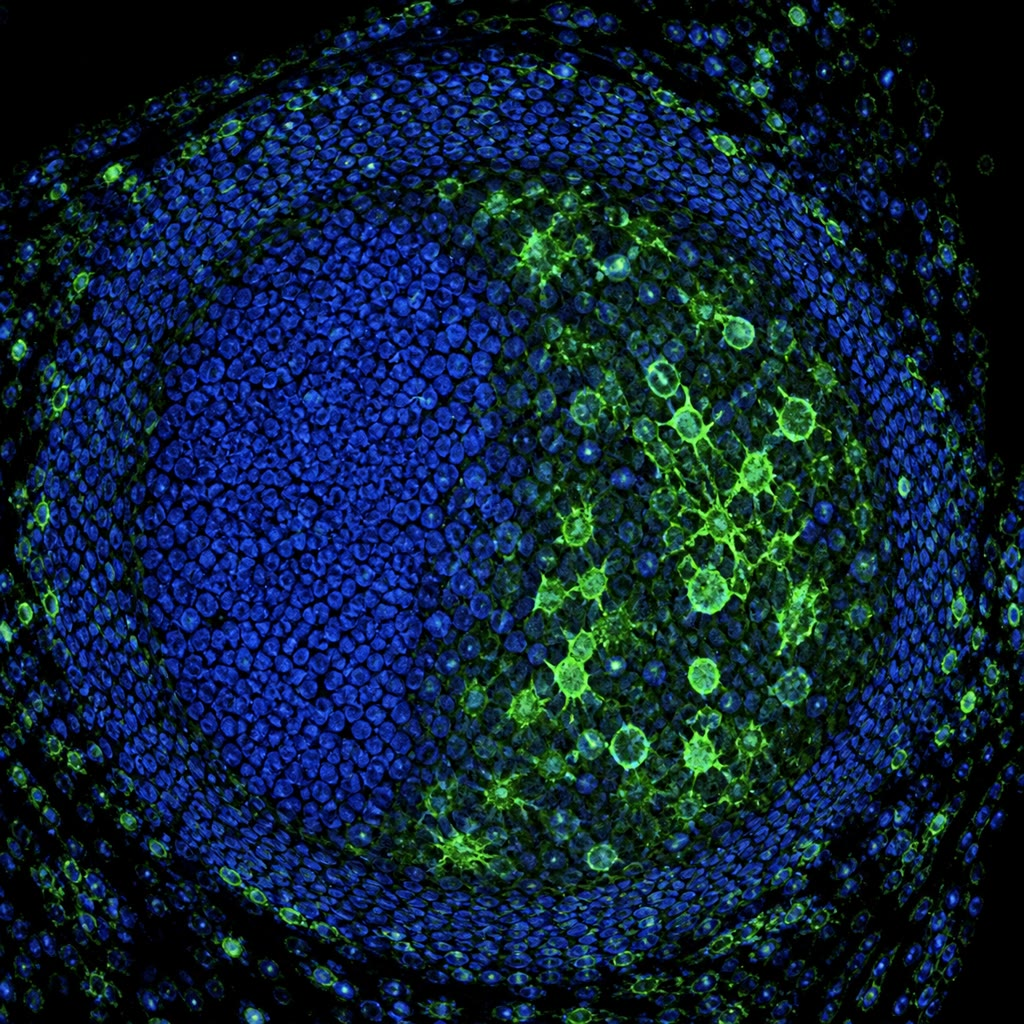
\includegraphics[width=0.36\linewidth]{images/book5/ai/b5-16-germinal-centre.jpg}\hspace{0.04\linewidth}
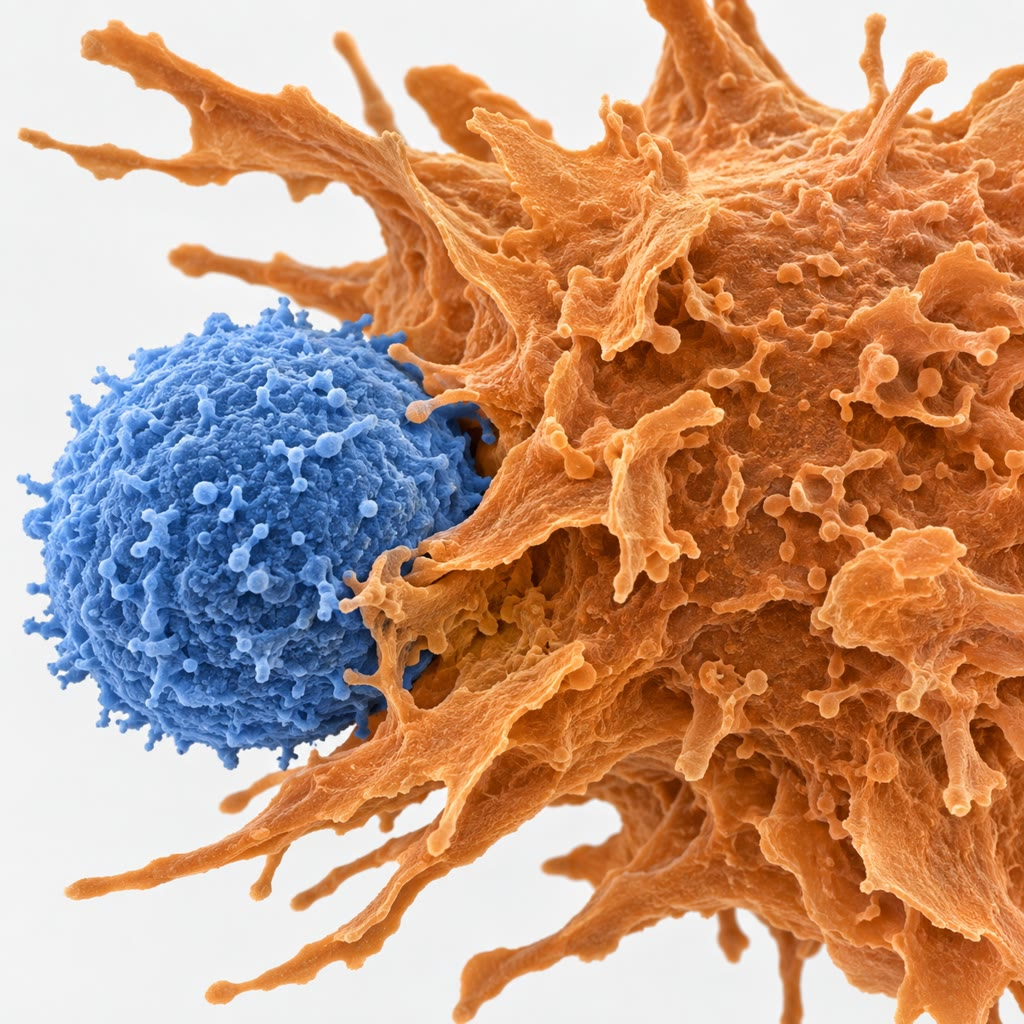
\includegraphics[width=0.36\linewidth]{images/book5/ai/b5-16-t-cell-apc.jpg}

{\small يسارًا: \omterm{def:b3:adaptive-immunity:germinal-centre}{مركز إنتاشي} في \omterm{def:b3:adaptive-immunity:lymphocytes}{عقدة لمفية} --- المنطقة
الداكنة المزدحمة ومنطقة الانتخاب الأفتح. ويمينًا: \omterm{def:b3:adaptive-immunity:lymphocytes}{لمفاوية
تائية} (صغيرة) ملامسة \omterm{def:b3:innate-immunity:innate}{لخلية تغصنية}، وهي اللحظة التي تُقرَّر
فيها الاستجابة التكيّفية.}
\end{omfigure}

\section{التحمل وإخفاقاته}

\begin{definition}[التحمل]\label{def:b3:adaptive-immunity:tolerance}
\index{تحمل مناعي}\index{انتخاب سالب}\index{توتة}\index{خمود}\index{FoxP3}\index{مناعة ذاتية}
تُصنع الذخيرة عشوائيًا فتحوي بالضرورة مستقبلات للذات.
و\emph{التحمل المركزي} يزيلها حيث تنضج الخلايا: ففي التوتة
تُقتل اللمفاويات التائية التي تربط مستقبلاتها ببتيد الذات
مع MHC ربطًا شديدًا (\emph{الانتخاب السالب})، وتُقتل أيضًا
التي لا تقدر على ربط MHC البتة (إذ تكون عديمة الفائدة)، ولا
يخرج إلا القليل المتوسط، بضع في المئة؛ ويجعل عامل استنساخ،
هو AIRE، خلايا التوتة تعبّر عن بروتينات من كل نسيج ---
الأنسولين، والغلوبولين الدرقي --- حتى تُحذف هناك اللمفاويات
التائية النوعية لها. واللمفاويات البائية التي تربط الذات في
النقي تُحذف أو تحرّر مستقبلاتها. و\emph{التحمل المحيطي}
يتولى الباقي: \omterm{def:b3:adaptive-immunity:lymphocytes}{فاللمفاوية التائية} التي تلقى مستضدها بلا
\omterm{def:b3:adaptive-immunity:response}{تحفيز مشارك} تُجعل غير مستجيبة (\emph{الخمود}) أو تُحذف؛
واللمفاويات التائية \emph{النظيمية}، التي يعرّفها العامل
FoxP3، تكبت كبتًا فاعلًا الاستجاباتِ \omterm{def:b3:adaptive-immunity:antibody}{ضد} الذات \omterm{def:b3:adaptive-immunity:antibody}{وضد} مستضدات
غير ضارة كالطعام والمعايشات. و\emph{المناعة الذاتية} هي
إخفاق هذه الضوابط: فداء السكري من النمط~1 (تهدم اللمفاويات
التائية خلايا $\beta$)، والتصلب المتعدد (المييلين)، \omterm{def:b3:innate-immunity:inflammation}{والتهاب}
المفاصل الرثوي (المفاصل)، والذئبة (أضداد \omterm{def:b3:adaptive-immunity:antibody}{ضد} مكوّنات نووية)،
وداء الدرق؛ ويرتبط كل منها بأليلات \omterm{def:b3:adaptive-immunity:mhc}{HLA} بعينها، تعرض ببتيدات
الذات ذات الصلة، ويطلق بعضَها خمجٌ بميكروب تشبه ببتيداته
بروتينًا ذاتيًا (الحمّى الرثوية بعد خمج بالمكورات العقدية).
\end{definition}

\begin{proof}[شواهد]
حقن ميداور (1953) خلايا من سلالة فئران نقية في وليدات من
سلالة أخرى؛ فلما بلغت قبلت المتلقيات طعوم جلد من سلالة
المتبرع كانت سترفضها لولا ذلك، بينما رفضت طعومًا من سلالات
ثالثة. فالتحمل مكتسب، ونوعي، ويحدده ما لقيه الجهاز المناعي
باكرًا --- وهو الأساس التجريبي لحذف برنت النسائلَ المتفاعلة
مع الذات. والأطفال الذين يولدون بلا مورّثة AIRE عاملة تنشأ
لديهم \omterm{def:b3:adaptive-immunity:tolerance}{مناعة ذاتية} \omterm{def:b3:adaptive-immunity:antibody}{ضد} أعضاء كثيرة دفعة واحدة؛ والذين بلا
\omterm{def:b3:adaptive-immunity:tolerance}{FoxP3} (وهي متلازمة نادرة مرتبطة بالصبغي X) تنشأ لديهم \omterm{def:b3:adaptive-immunity:tolerance}{مناعة
ذاتية} قاتلة في الرضاعة --- وهما ذراعا التحمل، كل منهما
مبيَّن بغيابه.
\end{proof}

\begin{example}[فرط الحساسية، والعوز، والزرع]\label{ex:b3:adaptive-immunity:failures}
\emph{الأرجية} استجابة Th2 \omterm{def:b3:adaptive-immunity:lymphocytes}{لمستضد} غير ضار --- طلع، أو فول
سوداني، أو بنسلين --- تنتج IgE؛ وعند إعادة التعرض يشابك
\omterm{def:b3:adaptive-immunity:lymphocytes}{المستضد} IgE على الخلايا البدينة، فتطلق الهيستامين في دقائق،
وإن كان \omterm{def:b3:adaptive-immunity:lymphocytes}{المستضد} في الدم كان الإطلاق الجهازي \emph{التأق}،
الذي يُعالَج بالأدرينالين. وأما \emph{العوز المناعي}:
فالأطفال الذين يفتقرون إلى \omterm{def:b3:adaptive-immunity:antibody}{RAG} أو إلى الإنزيم ADA لا يصنعون
لمفاويات (العوز المناعي المشترك الشديد) ويموتون من الخمج ما
لم يُعطوا نقيًا أو معالجة مورّثية؛ وHIV يهدم اللمفاويات
التائية CD4 ومعها المساعدة التي تحتاج إليها كل استجابة.
وأما \emph{الزرع}: فترى لمفاويات المتلقي التائية جزيئات \omterm{def:b3:adaptive-immunity:mhc}{HLA}
المتبرع غريبة، ويستجيب ما يصل إلى عُشر اللمفاويات التائية
كلها --- أي أكثر بكثير مما يستجيب لأي ممرض --- فتُطابَق
الطعوم عند مواضع \omterm{def:b3:adaptive-immunity:mhc}{HLA} ويُكبت المتلقي مناعيًا مدى الحياة؛
وطعم النقي قد يهاجم مضيفه الجديد بدل ذلك. وأما الاستعمالات
المقصودة: فالأضداد وحيدة النسيلة في
\cref{ch:b3:genetic-engineering}، ومثبطات نقاط التفتيش التي
تطلق اللمفاويات التائية \omterm{def:b3:adaptive-immunity:antibody}{ضد} الأورام
(\cref{ch:b3:cancer-biology})، واللمفاويات التائية المهندسة
بمستقبل خيمري \omterm{def:b3:adaptive-immunity:lymphocytes}{لمستضد} ورمي (CAR-T)، التي شفت ابيضاضات لم
يمسّها شيء آخر.
\end{example}

\section{التلقيح}

\begin{definition}[اللقاحات ومناعة القطيع]\label{def:b3:adaptive-immunity:vaccine}
\index{لقاح}\index{مناعة القطيع}\index{عدد التكاثر الأساسي}\index{نجاعة اللقاح}
\emph{اللقاح} يعرض مستضدات ممرض، مع \omterm{prop:b3:innate-immunity:bridge}{مادة مساعدة} أو في صورة
تثير المستقبلات الفطرية، فيكتسب المتلقي خلايا ذاكرة
وأضدادًا من غير المرض (و\cref{ch:b3:virology} يعدّد أنواعه).
و\emph{نجاعته} $E$ نسبة المُلقَّحين المحميين. وتمتد الحماية
إلى ما وراء المُلقَّحين: فالممرض الذي ينتشر في جمهرة تُعدي
فيها كل حالة $R_{0}$ حالة أخرى وسطيًا حين يكون الجميع
قابلين --- وهو \emph{عدد التكاثر الأساسي} --- لا يُعدي إلا
$R_{0}$ مضروبًا في نسبة القابلين حين يكون بعضهم مناعيًا،
ويزول حين يهبط ذلك العدد دون الواحد. وتلك \emph{مناعة
القطيع}: ففوق عتبة من المناعيين تنكسر سلسلة الانتقال ويُحمى
غير المُلقَّحين --- الرُّضّع، والمنقوصو المناعة، ومن أخفق
فيهم اللقاح --- بمن حولهم.
\end{definition}

\begin{theorem}[عتبة مناعة القطيع]\label{thm:b3:adaptive-immunity:herd}
\index{مناعة القطيع!العتبة}\index{نموذج SIR}
في جمهرة تكون فيها نسبة $p$ مناعية والباقي قابلًا، تُعدي كل
حالة وسطيًا $R_{\text{eff}} = R_{0}(1 -
p)$ حالة أخرى. ولا يمكن لوباء أن يبدأ إذا كان
$R_{\text{eff}} < 1$، أي إذا كان
\[
p > p_{c} = 1 - \frac{1}{R_{0}} .
\]
ومع \omterm{def:b3:adaptive-immunity:vaccine}{لقاح} نجاعته $E$ تكون التغطية اللازمة $f_{c} = p_{c}/E$.
وإذا جرى وباء فعلًا في جمهرة قابلة (\omterm{thm:b3:adaptive-immunity:herd}{نموذج SIR}، بمعدل خمج
$\beta$ ومعدل تعافٍ $\gamma$، حيث $R_{0} =
\beta/\gamma$)، فإنه يبلغ ذروته حين تهبط نسبة القابلين إلى
$1/R_{0}$، وتحقق النسبة التي لا تُخمج أبدًا، $s_{\infty}$،
العلاقة $\ln s_{\infty} = -R_{0}(1 - s_{\infty})$.
\end{theorem}
\begin{proof}
كل حالة تصنع تماسّات كانت ستُعدي $R_{0}$ شخصًا لو كان
الجميع قابلين؛ ونسبة $1 - p$ منهم قابلة، فيكون $R_{\text{eff}} =
R_{0}(1-p)$، ويعطي الشرط $R_{\text{eff}} < 1$ مقدار $p_{c}$؛
\omterm{def:b3:adaptive-immunity:vaccine}{ولقاح} يحمي نسبة $E$ ممن يتلقونه يجعل نسبة $Ef$ من الجمهرة
مناعية، فيلزم $Ef > p_{c}$. وفي \omterm{thm:b3:adaptive-immunity:herd}{نموذج SIR} يكون
$\mathrm{d}s/\mathrm{d}t = -\beta si$ و$\mathrm{d}i/\mathrm{d}t =
\beta si - \gamma i = \gamma i(R_{0}s - 1)$، فينمو $i$ ما دام $s >
1/R_{0}$ ويهبط بعد ذلك: فالذروة عند $s = 1/R_{0}$. وبقسمة
المعادلتين إحداهما على الأخرى، $\mathrm{d}i/\mathrm{d}s = -1 + 1/(R_{0}s)$، فيكون $i + s -
\ln s/R_{0}$ ثابتًا؛ وبحسابه عند البداية ($s = 1$، و$i
\approx 0$) وعند النهاية ($i = 0$، و$s = s_{\infty}$) نجد
$s_{\infty} - \ln s_{\infty}/R_{0} = 1$، وهي علاقة الحجم النهائي.
\end{proof}

\begin{example}[الحصبة والجدري]\label{ex:b3:adaptive-immunity:measles}
للحصبة $R_{0} \approx 15$: أي $p_{c} = 1 - 1/15 = 93\,\%$، ومع
\omterm{def:b3:adaptive-immunity:vaccine}{لقاح} نجاعته $97\,\%$ بعد جرعتين تكون التغطية اللازمة
$96\,\%$ --- ولذلك تعود الحصبة حيثما تراجع التلقيح بضع في
المئة، ولذلك يكون الطفل غير المُلقَّح في بلد جيد التلقيح
آمنًا مع ذلك. وكان للجدري $R_{0} \approx 5$--$7$، وعتبة قرب
$80$--$85\,\%$، ولا مستودع حيواني له، ولا حاملين بلا أعراض،
\omterm{def:b3:adaptive-immunity:vaccine}{ولقاح} ينجح بجرعة واحدة: فكان قابلًا للاستئصال، واستُؤصل.
وشلل الأطفال قريب من ذلك. وأما الإنفلونزا وفيروسات كورونا،
التي تنجرف مستضداتها (\cref{ch:b3:virology}) وتضعف المناعة
ضدها، فليست كذلك. وفي جمهرة غير مُلقَّحة يخمج وباء عند
$R_{0} = 3$، بعلاقة الحجم النهائي، $1 - s_{\infty} = 94\,\%$
من الناس؛ وعند $R_{0} = 1.5$، $58\,\%$.
\end{example}

\begin{omfigure}
\begin{tikzpicture}
\begin{axis}[
  width=6.4cm, height=5.4cm,
  axis x line=bottom, axis y line=left,
  xmin=1, xmax=18, ymin=0, ymax=1,
  xlabel={$R_{0}$}, ylabel={العتبة $p_{c}$},
  xlabel style={font=\small, at={(axis description cs:0.5,-0.12)}, anchor=north}, ylabel style={font=\small},
  tick label style={font=\scriptsize}, xtick={1,3,6,9,12,15,18}, ytick={0,0.5,0.8,0.93,1}, yticklabels={0,0.5,0.8,0.93,1},
  clip=false,
]
\addplot[very thick, omDef, domain=1:18, samples=80] {1-1/x};
\fill[omThm] (axis cs:15,0.933) circle (2pt); \node[font=\scriptsize, anchor=south east] at (axis cs:15,0.94) {الحصبة};
\fill[omThm] (axis cs:6,0.833) circle (2pt); \node[font=\scriptsize, anchor=north west] at (axis cs:6.3,0.82) {الجدري};
\fill[omThm] (axis cs:2.5,0.6) circle (2pt); \node[font=\scriptsize, anchor=north west] at (axis cs:2.6,0.58) {إنفلونزا 1918};
\end{axis}
\begin{axis}[
  at={(7.6cm,0)}, anchor=south west,
  width=6.4cm, height=5.4cm,
  axis x line=bottom, axis y line=left,
  xmin=0, xmax=60, ymin=0, ymax=0.35,
  xlabel={أيام}, ylabel={نسبة المعدين},
  xlabel style={font=\small, at={(axis description cs:0.5,-0.12)}, anchor=north}, ylabel style={font=\small},
  tick label style={font=\scriptsize}, xtick={0,20,40,60}, ytick={0,0.1,0.2,0.3},
  clip=false,
]
\addplot[very thick, omThm, smooth] coordinates {(0,0.001) (5,0.003) (10,0.012) (15,0.04) (20,0.12) (25,0.25) (28,0.30) (31,0.27) (35,0.18) (40,0.09) (45,0.04) (50,0.015) (55,0.006) (60,0.002)};
\addplot[very thick, omDef, smooth] coordinates {(0,0.001) (5,0.0015) (10,0.0025) (15,0.004) (20,0.006) (25,0.009) (30,0.012) (35,0.014) (40,0.015) (45,0.014) (50,0.012) (55,0.009) (60,0.007)};
\node[font=\scriptsize, omThm, anchor=west] at (axis cs:30,0.3) {بلا مناعة، $R_{0} = 3$};
\node[font=\scriptsize, omDef, anchor=south west] at (axis cs:32,0.03) {\qty{60}{\%} مُلقَّحون: $R_{\text{eff}} = 1.2$};
\end{axis}
\end{tikzpicture}

{\small يسارًا: العتبة $1 - 1/R_{0}$ --- فكلما كان المرض
أشد عدوى وجب أن يكون المناعيون أقرب إلى الجميع. ويمينًا:
وباء SIR عند $R_{0} = 3$ في جمهرة ساذجة وفي جمهرة \qty{60}{\%}
منها مناعي، وهي نسبة لا تكفي لوقفه لكنها تفلطحه وتبطئه.}
\end{omfigure}

\begin{omfigure}
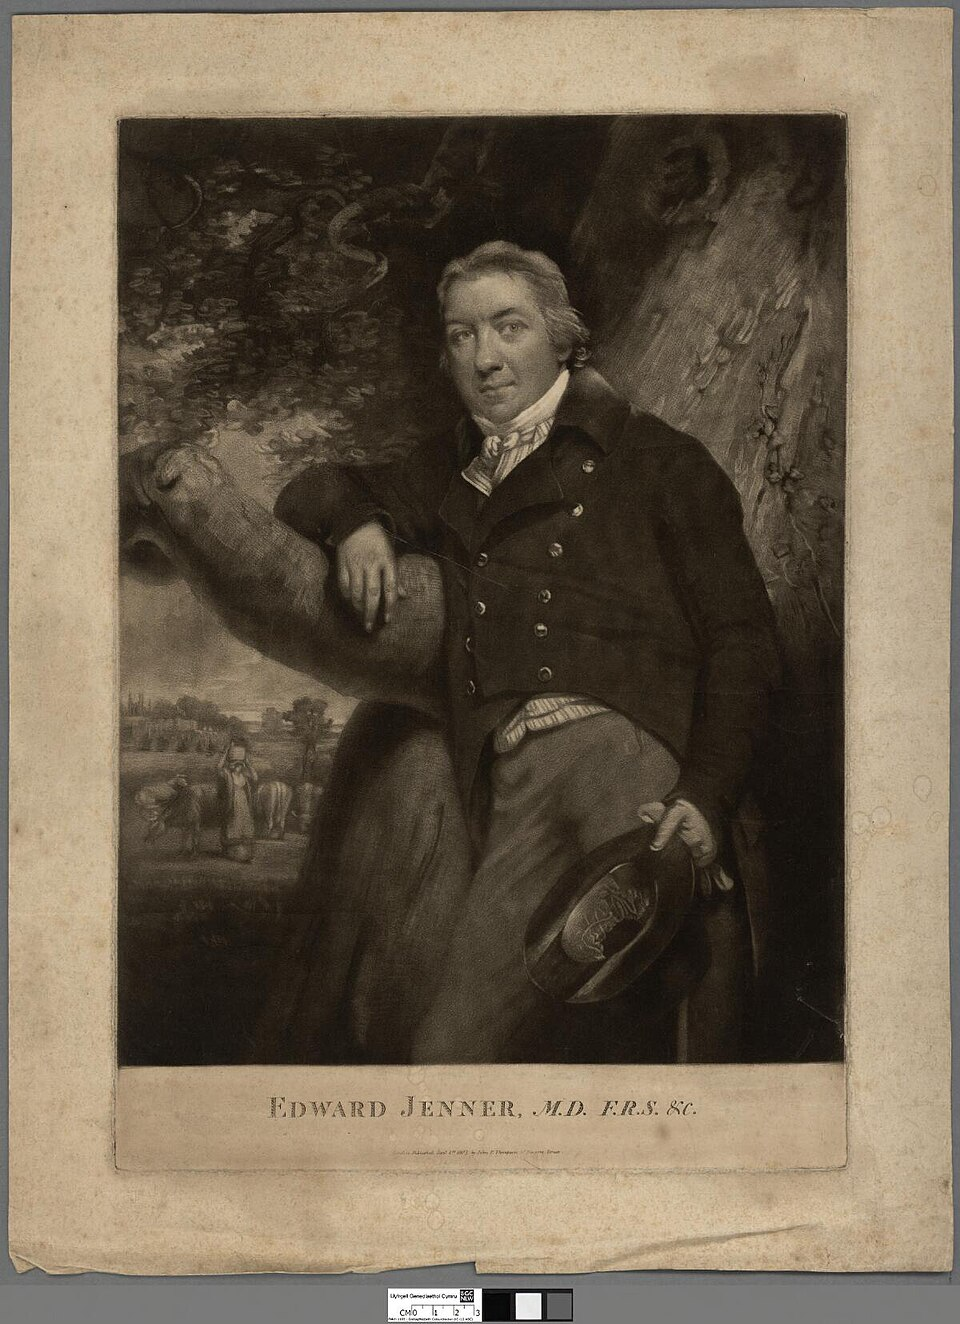
\includegraphics[width=0.30\linewidth]{images/book5/jenner.jpg}\hspace{0.04\linewidth}

\includegraphics[width=0.50\linewidth]{images/book5/ai/b5-16-vaccination.jpg}

{\small إدوارد جينر، الذي حمى صبيًا عام 1796 من الجدري بجدري
البقر فأسس التلقيح (نقش من 1807، ملكية عامة). ويمينًا: الفعل
نفسه بعد قرنين --- \omterm{def:b3:adaptive-immunity:vaccine}{لقاح} عضلي ستحمل الخلايا التغصنية في
الدالية مستضده إلى العقد اللمفية الإبطية.}
\end{omfigure}

\begin{remark}[ما تتذكره المناعة]\label{rem:b3:adaptive-immunity:memory}
الجهاز المناعي التكيّفي آلة داروينية داخل كل واحد منا: تباين
عشوائي (V(D)J، والطفور المفرط)، وانتخاب (\omterm{def:b3:adaptive-immunity:lymphocytes}{بالمستضد}، في \omterm{def:b3:adaptive-immunity:germinal-centre}{المركز
الإنتاشي}، \omterm{def:b3:adaptive-immunity:antibody}{وضد} الذات في \omterm{def:b3:adaptive-immunity:tolerance}{التوتة})، ووراثة (خلايا الذاكرة،
والتوسع النسيلي). وهو يحل في أسابيع المشكلة التي يحلها
التطور في آلاف السنين --- جزيء يربط هدفًا لم يُرَ من قبل
--- وأجوبته من أفضل ما دُرس من حالات التطور الملاحَظ
مباشرةً. وثمنه \omterm{def:b3:adaptive-immunity:tolerance}{المناعة الذاتية}، واعتماده على حكم الجهاز
الفطري تام، وذاكرته، التي استغلها جينر وتكتبها اللقاحات
عمدًا، هي سبب قدرة نوع من الحيوانات طويلة العمر بطيئة
التوالد على البقاء في عالم من ميكروبات سريعة التوالد.
\end{remark}

\section{تمارين}

\begin{exercise}[$\star$]\label{exo:b3:adaptive-immunity:1}
اذكر أركان \omterm{def:b3:adaptive-immunity:lymphocytes}{الانتخاب النسيلي} الأربعة والتجربة التي تدعم
كلًّا من الأولين.
\end{exercise}

\begin{exercise}[$\star$]\label{exo:b3:adaptive-immunity:2}
صف بنية \omterm{def:b3:adaptive-immunity:antibody}{الضد} واذكر وظيفة كل صنف من الأصناف الخمسة.
\end{exercise}

\begin{exercise}[$\star$]\label{exo:b3:adaptive-immunity:3}
قابل بين \omterm{def:b3:adaptive-immunity:mhc}{MHC من الصنف~I} والصنف~II في توزع الخلايا، ومصدر
الببتيد، وطول الببتيد، \omterm{def:b3:adaptive-immunity:lymphocytes}{واللمفاوية التائية} التي تقرأ كلًّا منهما.
\end{exercise}

\begin{exercise}[$\star$]\label{exo:b3:adaptive-immunity:4}
عرّف $R_{0}$ وعتبة \omterm{def:b3:adaptive-immunity:vaccine}{مناعة القطيع}، واحسب العتبة للنكاف
($R_{0} = 5$)، والسعال الديكي ($R_{0} = 12$)، وإنفلونزا
1918 ($R_{0} = 2.5$).
\end{exercise}

\begin{exercise}[$\star\star$]\label{exo:b3:adaptive-immunity:5}
لنوع $V_{H} = 50$، و$D = 20$، و$J_{H} = 5$، وموضع خفيف واحد
عند $V = 60$ و$J = 4$. احسب الذخيرة التوفيقية، ثم المجموع
بعامل وصلي قدره $10^{4}$. وكيف يقارَن ذلك بعدد اللمفاويات
البائية $10^{9}$ التي في الحيوان؟
\end{exercise}

\begin{exercise}[$\star\star$]\label{exo:b3:adaptive-immunity:6}
المنطقة المتغيرة في \omterm{def:b3:adaptive-immunity:lymphocytes}{لمفاوية بائية} في \omterm{def:b3:adaptive-immunity:germinal-centre}{مركز إنتاشي} \qty{1000}{bp}؛
ويطفّر AID بمعدل $10^{-3}$ لكل زوج أساس في الانقسام. فعلى مدى
$20$ انقسامًا، كم طفرة في الخلية، وبين $10^{5}$ خلية كم
متغيرًا متمايزًا أحادي الأساس من \omterm{def:b3:adaptive-immunity:antibody}{الضد} يتولد؟ وقارن ذلك
بالبدائل الأحادية الممكنة البالغة $3000$.
\end{exercise}

\begin{exercise}[$\star\star$]\label{exo:b3:adaptive-immunity:7}
اشرح لماذا لا تتعرف \omterm{def:b3:adaptive-immunity:lymphocytes}{لمفاوية تائية} من شخص ببتيدات فيروسية
تعرضها خلايا شخص آخر، ولماذا تجعل هذه الحقيقة نفسها الزرع
صعبًا وجهاز \omterm{def:b3:adaptive-immunity:mhc}{HLA} متعدد الأشكال.
\end{exercise}

\begin{exercise}[$\star\star$]\label{exo:b3:adaptive-immunity:8}
تنبأ بالنمط المناعي الظاهري لطفل يفتقر إلى (أ) RAG1، و(ب)
AIRE، و(ج) \omterm{def:b3:adaptive-immunity:tolerance}{FoxP3}، و(د) إنزيم \omterm{def:b3:adaptive-immunity:antibody}{تبديل الصنف} AID، و(ه) اللمفاويات التائية CD4.
\end{exercise}

\begin{exercise}[$\star\star$]\label{exo:b3:adaptive-immunity:9}
\omterm{def:b3:adaptive-immunity:vaccine}{لقاح} نجاعته \qty{90}{\%} ومرض $R_{0} = 6$. فأي تغطية توقف
الانتقال؟ وإذا كانت التغطية \qty{80}{\%}، فما
$R_{\text{eff}}$، وأي نسبة من الجمهرة يخمجها وباء (استعمل
علاقة الحجم النهائي بعد استبدال $R_{0}$ بالعدد
$R_{\text{eff}}$ بين القابلين --- أو بيّن لماذا يكون ذلك صحيحًا تقريبًا)؟
\end{exercise}

\begin{exercise}[$\star\star\star$]\label{exo:b3:adaptive-immunity:10}
استنتج علاقة الحجم النهائي في المبرهنة من معادلات SIR
وحلّها عدديًا عند $R_{0} = 1.5$، و$2$، و$3$، و$5$. ولماذا لا
يخمج وباء الجميع أبدًا حتى بلا أي تدخل؟
\end{exercise}

\begin{exercise}[$\star\star\star$]\label{exo:b3:adaptive-immunity:11}
يرفع \omterm{def:b3:adaptive-immunity:germinal-centre}{نضج الألفة} الربط ألف ضعف في ثلاثة أسابيع. عامِل \omterm{def:b3:adaptive-immunity:germinal-centre}{المركز
الإنتاشي} جمهرةً تحت الانتخاب: فمع معدل طفر قدره واحد في
الخلية في الانقسام، ونسبة $10^{-2}$ من الطفرات تحسّن الألفة
بعامل $1.5$ والباقي محايد أو ضار، كم جولة انتخاب تلزم لكسب
ألف ضعف، وكم خلية يجب أن تفحص كل جولة؟ وعلّق على سبب تنظيم
\omterm{def:b3:adaptive-immunity:germinal-centre}{المركز الإنتاشي} في دورات.
\end{exercise}

\begin{exercise}[$\star\star\star$]\label{exo:b3:adaptive-immunity:12}
أمراض \omterm{def:b3:adaptive-immunity:tolerance}{المناعة الذاتية} أشيع في النساء وترتبط بأليلات \omterm{def:b3:adaptive-immunity:mhc}{HLA}؛ وقد
ارتفع داء السكري من النمط~1 خمسة أضعاف في خمسين سنة في
البلدان الغنية. اقترح، بآليات هذا الفصل
و\cref{ch:b3:microbiomes}، تفسيرات لكل ملاحظة واختبارًا
واحدًا لكل تفسير.
\end{exercise}

\section{مسألة: حملة تلقيح}

\begin{problem}[{مسألة نهاية الأسبوع --- ذخيرة تُعدّ، واستجابة
تُوقَّت من مئة خلية إلى ميليلتر من المصل، ومركز إنتاشي
يُشغَّل خوارزميةً تطورية، وحملة حصبة تُخطَّط في مواجهة عتبة
القطيع، وتُختم بحجم الذخيرة، وبالضد الذي تصنعه خلايا بلازمية
في يوم، وبالتغطية التي يحتاج إليها بلد}]
\label{pb:b3:adaptive-immunity:1}
المعطيات: $V_{H} = 40$، و$D = 25$، و$J_{H} = 6$؛ وموضعان
خفيفان $(40, 5)$ و$(30, 4)$؛ وعامل وصلي $3\times 10^{4}$. وفي
الجسم $10^{11}$ \omterm{def:b3:adaptive-immunity:lymphocytes}{لمفاوية بائية}؛ وواحدة في $10^{5}$ تربط حاتمة
بعينها؛ وتُجنَّد $100$ سليفة؛ والانقسام كل \qty{8}{h} مدة
$7$ أيام؛ و\qty{30}{\%} من النسيلة تصير خلايا بلازمية تفرز
كل منها $2000$ جزيء IgG في الثانية؛ وكتلة IgG
\qty{150}{kDa}؛ وحجم البلازما \qty{3}{L}؛ وعمر نصف IgG
\qty{21}{d}. \omterm{def:b3:adaptive-immunity:germinal-centre}{والمركز الإنتاشي}: منطقة متغيرة \qty{1000}{bp}،
و$10^{-3}$ طفرة لكل زوج أساس في الانقسام، وواحدة في $100$
من الطفرات تحسّن الألفة بعامل $1.5$. والحصبة: $R_{0} = 15$،
\omterm{def:b3:adaptive-immunity:vaccine}{ونجاعة اللقاح} $0.93$ بعد جرعة واحدة و$0.97$ بعد جرعتين؛
وبلد فيه $5\times 10^{6}$ نسمة و$60\,000$ ولادة في السنة.

\medskip
\noindent\textbf{الجزء الأول --- الذخيرة.}
\begin{enumerate}
  \item احسب الذخيرة التوفيقية والمجموع مع \omterm{def:b3:adaptive-immunity:antibody}{التنوع الوصلي}.
  \item قارن ذلك بعدد اللمفاويات البائية. فأي نسبة من
        الذخيرة الممكنة يعبّر عنها جسم واحد في وقت واحد،
        وماذا يتبع ذلك بالنسبة إلى ذخيرتي شخصين؟
  \item كم \omterm{def:b3:adaptive-immunity:lymphocytes}{لمفاوية بائية} في الجسم تربط الحاتمة؟ وكم منها
        وسطيًا في \omterm{def:b3:adaptive-immunity:lymphocytes}{عقدة لمفية} فيها $10^{8}$ \omterm{def:b3:adaptive-immunity:lymphocytes}{لمفاوية بائية}؟
  \item في الوليد $10^{9}$ \omterm{def:b3:adaptive-immunity:lymphocytes}{لمفاوية بائية}. فكم منها يربط
        الحاتمة، ولماذا تكون استجابة الوليد ضعيفة مع ذلك؟
  \item العروة الثالثة في السلسلة الثقيلة من \omterm{def:b3:adaptive-immunity:antibody}{الضد} يصنعها
        \omterm{def:b3:adaptive-immunity:antibody}{التنوع الوصلي}. اشرح لماذا تكون هذه العروة أشد أجزاء
        الجزيء تغيرًا وتقع عادةً في مركز موقع الربط.
  \item يضيف \omterm{def:b3:adaptive-immunity:germinal-centre}{الطفور الجسدي المفرط} تنوعًا بعد الانتخاب،
        ويضيفه V(D)J قبله. فلماذا يفيد وجود الاثنين، بهذا
        الترتيب؟
\end{enumerate}

\medskip
\noindent\textbf{الجزء الثاني --- الاستجابة.}
\begin{enumerate}[resume]
  \item انطلاقًا من $100$ خلية تنقسم كل \qty{8}{h}، كم تصير
        بعد $7$ أيام؟ وكم \omterm{def:b3:adaptive-immunity:response}{خلية بلازمية}؟
  \item كم جزيء IgG تفرزه في اليوم، وما كتلته؟ وأي تركيز
        مصلي يعطيه إنتاج يوم واحد في \qty{3}{L}؟
  \item بعد عشرة أيام من الإفراز بذلك المعدل، وبإهمال
        الانحلال، ما التركيز بوحدة g/L؟ وقارنه بمجموع IgG
        السويّ البالغ \qty{10}{g/L}.
  \item تموت الخلايا البلازمية بعد أسبوعين؛ ثم ينحل \omterm{def:b3:adaptive-immunity:antibody}{الضد}
        بعمر نصف \qty{21}{d}. فكم يلزم حتى يهبط تركيز
        السؤال 9 مئة ضعف؟ وما الذي يصون \omterm{def:b3:adaptive-immunity:antibody}{الضد} سنين؟
  \item تبدأ استجابة ثانوية من $10^{5}$ \omterm{def:b3:adaptive-immunity:response}{خلية ذاكرة}. فكم خلية
        بعد $3$ أيام، وكيف يقارَن ذلك بالاستجابة الأولية في
        اليوم 3 واليوم 7؟
  \item اشرح لماذا يأتي IgM أولًا وIgG لاحقًا في استجابة
        أولية، ولماذا تكون الاستجابة الثانوية IgG من البداية.
\end{enumerate}

\medskip
\noindent\textbf{الجزء الثالث --- \omterm{def:b3:adaptive-immunity:germinal-centre}{المركز الإنتاشي}.}
\begin{enumerate}[resume]
  \item كم طفرة تكتسب \omterm{def:b3:adaptive-immunity:lymphocytes}{لمفاوية بائية} في منطقتها المتغيرة في
        الانقسام الواحد؟ وعلى مدى $20$ انقسامًا؟
  \item أي نسبة من بنات انقسام واحد تحمل طفرة محسِّنة؟ وفي
        \omterm{def:b3:adaptive-immunity:germinal-centre}{مركز إنتاشي} فيه $10^{4}$ خلية منقسمة، كم خلية
        محسَّنة تظهر في كل انقسام؟
  \item كم تحسينًا متتاليًا بعامل $1.5$ يعطي كسبًا ألف ضعف
        في الألفة؟ وإذا استغرقت كل جولة انتخاب انقسامين
        (\qty{12}{h})، فكم يكون ذلك من الزمن؟
  \item معظم الطفرات تضر \omterm{def:b3:adaptive-immunity:antibody}{الضد}. فإذا هدمت \qty{50}{\%} من
        الطفرات الربطَ، أي نسبة من الخلايا تنجو من طفر كل
        انقسام، ولماذا يجب أن تقتل المنطقة الفاتحة معظم
        الخلايا؟
  \item \omterm{def:b3:adaptive-immunity:vaccine}{لقاح} يُعطى جرعتين بينهما ستة أسابيع يعطي أضدادًا
        أعلى ألفة من جرعة واحدة. اشرح ذلك \omterm{def:b3:adaptive-immunity:germinal-centre}{بالمركز الإنتاشي}.
  \item بعض الفيروسات (HIV، والإنفلونزا) تهرب من الأضداد
        بتطفير سطحها. اشرح لماذا يبقى \omterm{def:b3:adaptive-immunity:germinal-centre}{المركز الإنتاشي} مع ذلك
        أساس الأمل في \omterm{def:b3:adaptive-immunity:vaccine}{لقاح} واسع الحماية.
\end{enumerate}

\medskip
\noindent\textbf{الجزء الرابع --- الحملة.}
\begin{enumerate}[resume]
  \item عتبة القطيع للحصبة، والتغطية المطلوبة بجرعة واحدة؛
        وبجرعتين.
  \item يلقّح البلد \qty{90}{\%} من الأطفال بجرعتين. فما
        نسبة المناعيين، وما $R_{\text{eff}}$، وما الحكم: هل
        تدور الحصبة؟
  \item كم قابلًا يتراكم في كل سنة من الولادات عند تغطية
        \qty{90}{\%} (غير المُلقَّحين مع إخفاقات \omterm{def:b3:adaptive-immunity:vaccine}{اللقاح})؟
        وبعد خمس سنين بلا حصبة، كم يكون عدد القابلين، ولماذا
        يسبب استيراد حالة عندئذ فاشية؟
  \item استعمل علاقة الحجم النهائي مع عدد التكاثر الفعال بين
        القابلين لتقدير النسبة التي تخمجها فاشية من أولئك
        القابلين. (خذ $R_{\text{eff}}$ من السؤال 20 عدد تكاثر
        في الجمهرة كلها، ولاحظ أن المرض ينتشر بين مجموع
        القابلين كأن $R_{0}$ هو $R_{\text{eff}}$.)
  \item تُرفع التغطية إلى \qty{95}{\%} بجرعتين. فما نسبة
        المناعيين وما $R_{\text{eff}}$؛ وهل تُبلَغ العتبة؟
  \item الرُّضّع دون السنة لا يمكن تلقيحهم \omterm{def:b3:adaptive-immunity:antibody}{ضد} الحصبة وهم
        أرجح من يموت بها. اشرح كيف تحميهم الحملة، وماذا يحدث
        لحمايتهم إذا هبطت التغطية إلى \qty{85}{\%}.
  \item لخّص: مجموع الذخيرة (السؤال~1)، وIgG الذي تصنعه
        خلايا بلازمية في يوم (السؤال~8)، والتغطية بجرعتين
        التي يحتاج إليها البلد (السؤال~19).
\end{enumerate}
\end{problem}
